\documentclass[12pt,a4paper]{beamer}
\usepackage[utf8]{vietnam}
\usepackage{amsmath}
\usepackage{amssymb}
\usepackage{graphicx}
\usepackage{lmodern}
\usetheme{CambridgeUS}
\usepackage{multicol}


\begin{document}
	\title{Mạch cộng hai số có 2 chữ số sử dụng các IC số}
	\author{Vũ Đức Cường 20202313, Lê Xuân Đức 20191759, Đỗ Công Hiếu 20202620, Hoàng Anh Tú 20164460}
	\date{Ngày 17 tháng 6 năm 2022}
\begin{frame}[plain]
	\maketitle
\end{frame}


\begin{frame}
	\frametitle{Nội dung}
	\tableofcontents[sections={1-3}]
\end{frame}
\begin{frame}
	\frametitle{Nội dung}
	\tableofcontents[sections={4-5}]
\end{frame}
\begin{frame}
	\frametitle{Nội dung}
	\tableofcontents[sections={6-7}]
\end{frame}
\subsection{Sơ lược về bài toán và mạch thiết kế}
\section{Tổng quan}
\begin{frame}
	\frametitle{Tổng quan}
	
	\begin{minipage}{5cm}
		\begin{itemize}
			\item Thiết kế một mạch để cộng hai số có 2 chứ số, kết quả trả về có thể là số có 3 chữ số.
			\item Mạch sử dụng các IC số, không sử dụng Vi điều khiển
			\item Nếu tính ra số bit để thực hiện phép tính thì cần ít nhất 8 bit, tuy nhiên ở đây chỉ làm việc với các IC 4 bit
		\end{itemize}
	\end{minipage}
	\hfill
	\begin{minipage}{6cm}
		\begin{center}
			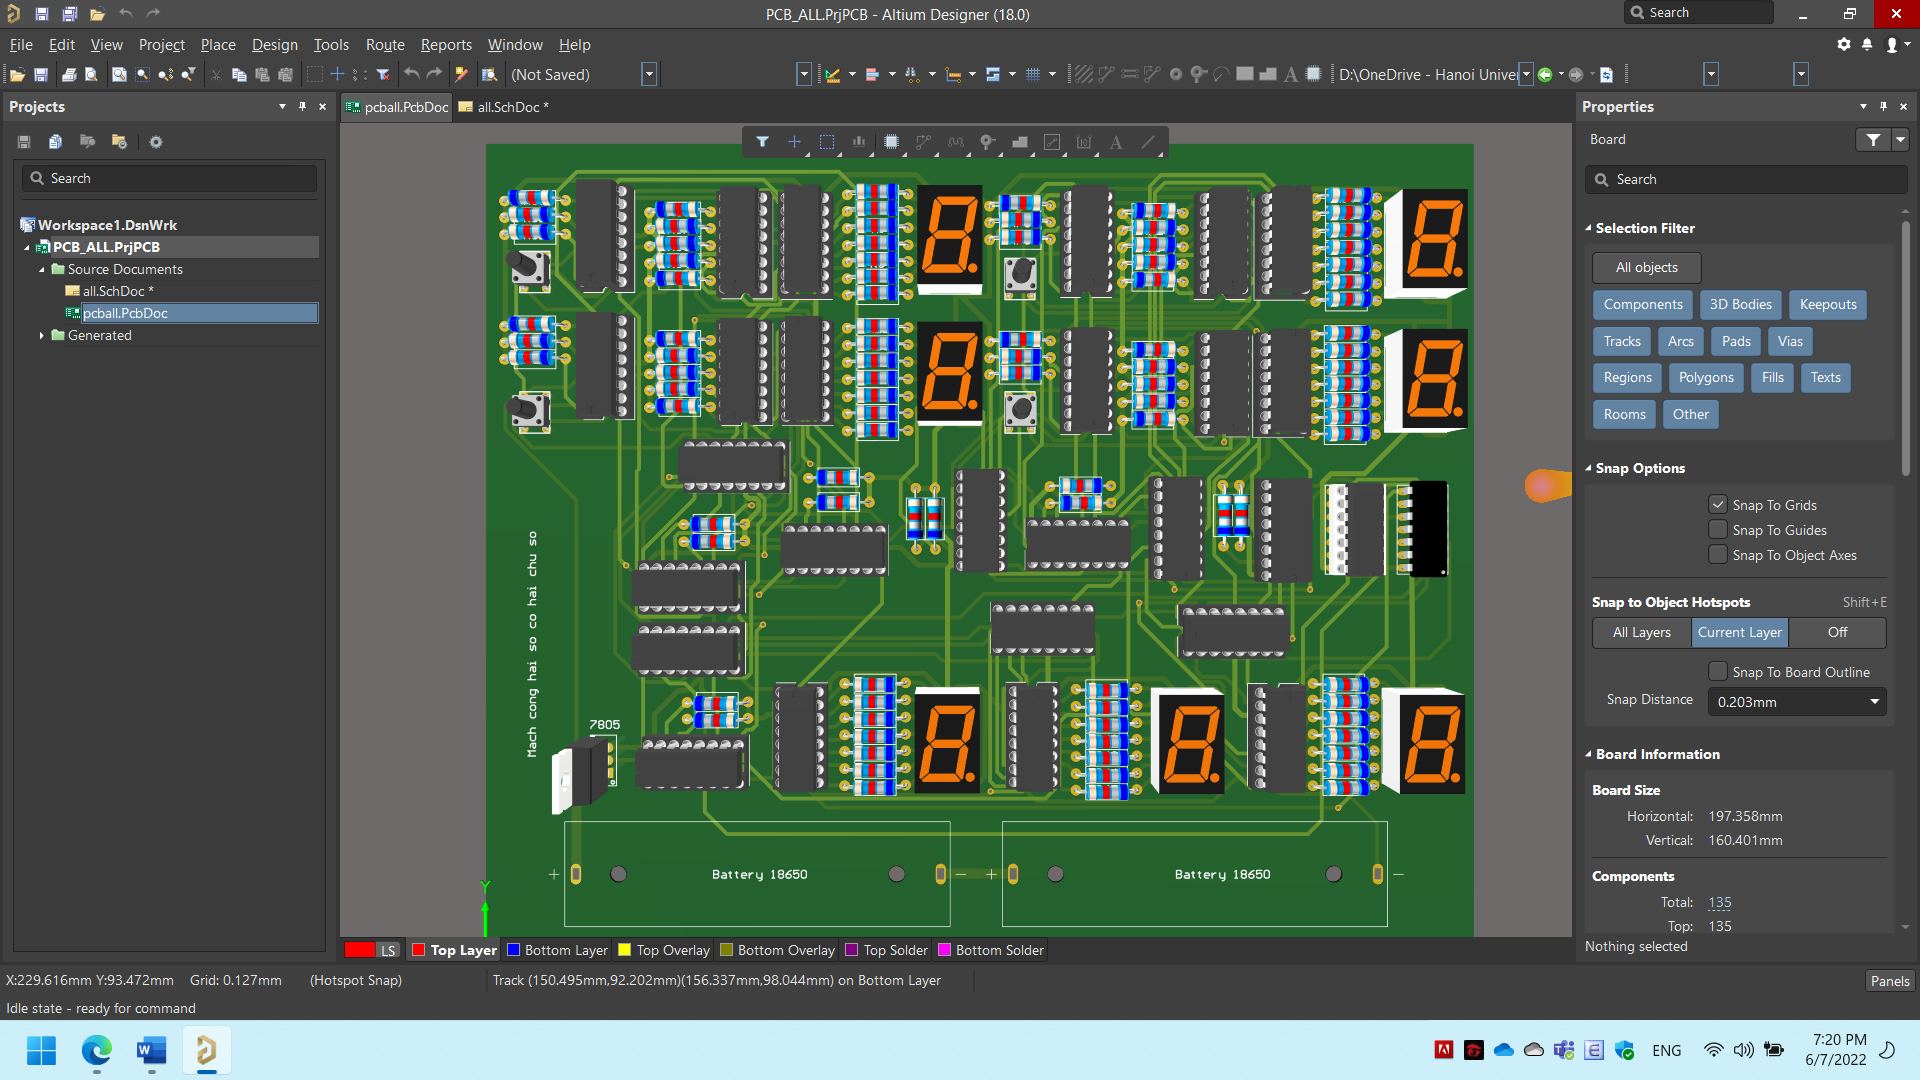
\includegraphics[width=1\linewidth]{img_all}
			\textit{{Hình ảnh thiết kế mạch trên Altium}}
		\end{center}
	\end{minipage}
\end{frame}




\begin{frame}
	\frametitle{Tổng quan}
	\framesubtitle{Sơ đồ khối hệ thống}
	\subsection{Sơ đồ khối}
	\begin{center}
		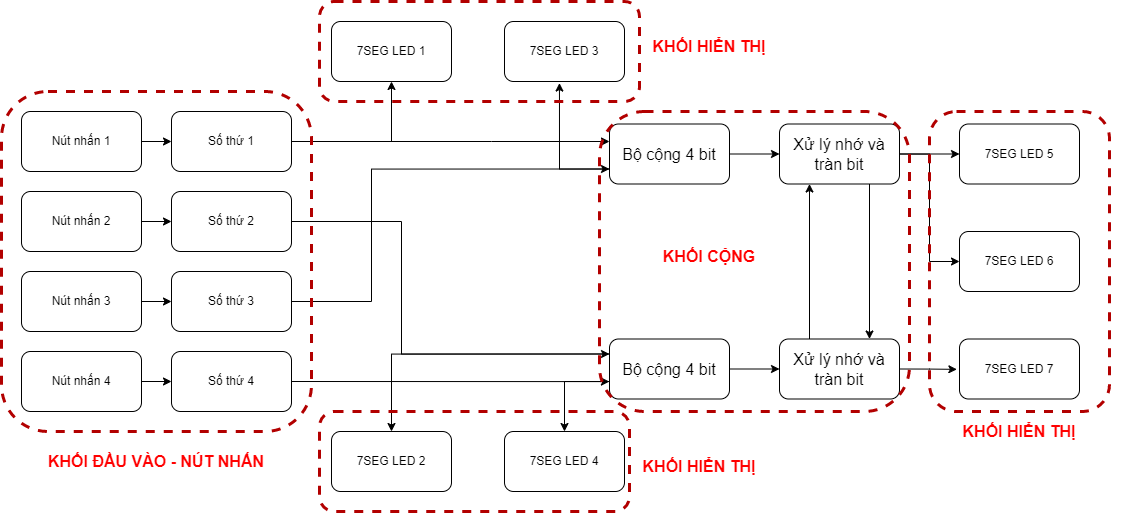
\includegraphics[width=1\linewidth]{sodo}
		\textit{Sơ đồ khối của hệ thống}
	\end{center}
\end{frame}



\section{Khối hiển thị}
\subsection{LED 7 segment}

\begin{frame}
	\frametitle{Khối hiển thị}
	\framesubtitle{LED 7 segment}
	\begin{minipage}{6cm}
		\includegraphics[width=1.3\linewidth]{image/led7doan}
		\includegraphics[width=1.3\linewidth]{image/led7doan_hienthi}\\
	\end{minipage}
	\hfill
	\begin{minipage}{5cm}
		\begin{center}
			\includegraphics[width=0.6\linewidth]{image/led7doanimg}
		\end{center}
	\end{minipage}
	\begin{center}
		\textit{Sơ đồ LED 7 đoạn}
	\end{center}
\end{frame}


\subsection{IC 74LS247}
\begin{frame}
	\frametitle{Khối hiển thị}
	\framesubtitle{IC 74LS247}
	
	\begin{minipage}{7cm}
		\begin{center}
			\includegraphics[width=1\linewidth]{image/74ls247}\\
			\textit{ Sơ đồ chân của IC 74LS247\\
				(TOP VIEW)}
		\end{center}
	\end{minipage}
	\hfill
	\begin{minipage}{4cm}
		\begin{flushleft}
			\includegraphics[width=1.2\linewidth]{image/74ls247img}
		\end{flushleft}
	\end{minipage}
\vspace{0.2cm}\\
IC là một bộ giải mã 4 bit thành tín hiệu điều khiển led 7 đoạn
\end{frame}


\begin{frame}
	\frametitle{Khối hiển thị}
	\framesubtitle{Mô phỏng Proteus với IC}
	\begin{center}
		\includegraphics[width=0.7\linewidth]{image/prt74247}\\
		\textit{Thực hiện mô phỏng Proteus với IC}
	\end{center}
\end{frame}

\subsection{Schematic khối hiển thị}

\begin{frame}
	\frametitle{Khối hiển thị}
	\framesubtitle{Schematic khối hiển thị}
	
	\begin{center}
		\includegraphics[width=0.8\linewidth]{image/sodonguyenlykhoicong}\\
		\textit{Sơ đồ nguyên lý khối hiển thị}
	\end{center}
\end{frame}

\section{Khối nút nhấn}

\subsection{IC 74LS76 Dual JK Flip Flop}
\begin{frame}
	
	\frametitle{Khối nút nhấn}
	\framesubtitle{IC 74LS76 Dual JK Flip Flop}
	
	Mỗi IC như thế này bao gồm 2 bộ JKFF độc lập nhau\\
	Chập 2 chân J và K của Flip Flop này ta được T Flip Flop
	\begin{center}
		\includegraphics[width=0.6\linewidth]{image/74ls76_symbol}\\
	\textit{Sơ đồ chân IC 74LS76 (5: VCC; 13: GND)}
	\end{center}
\end{frame}
\subsection{Nút nhấn}
\begin{frame}
	\frametitle{Khối nút nhấn}
	\framesubtitle{Nút nhấn}
	
	Nút nhấn này như là một công tắc hành trình, 2 đầu dây cạnh nhau sẽ thông mạch khi nút được nhấn giữ, và ngược lại.
	\begin{center}
		\includegraphics[width=0.5\linewidth]{image/button}\\
		\textit{Nút nhấn (công tắc hành trình)}
	\end{center}
\end{frame}

\begin{frame}
	\frametitle{Khối nút nhấn}
	\framesubtitle{Mô phỏng Proteus với mạch Flip Flop }
	Bằng cách mắc nối tiếp 2 IC 74LS76, tương đương 4 bộ JKFF ta được một bộ đếm:
	\begin{center}
		\includegraphics[width=1\linewidth]{image/prt7476}\\
		\textit{Đếm từ 0 $\to$ 15 sử dụng 4 JK FilpFlop}
	\end{center}
\end{frame}
\subsection{IC 74LS85}
\begin{frame}
	\frametitle{Khối nút nhấn}
	\framesubtitle{IC 74LS85}
	
	IC là bộ so sánh 2 số 4 bit, trả về kết quả =, > hoặc <
	\begin{minipage}{6cm}
		\begin{center}
			\includegraphics[width=1\linewidth]{image/74ls85}
		\end{center}
	\end{minipage}
	\hfill
	\begin{minipage}{4cm}
		\begin{flushleft}
			\includegraphics[width=1\linewidth]{image/74ls85img}
		\end{flushleft}
	\end{minipage}
	\begin{center}
		\textit{Sơ đồ chân 74LS85 (TOP VIEW)}
	\end{center}
\end{frame}

\begin{frame}
	\frametitle{Khối nút nhấn}
	\framesubtitle{Mô phỏng Protues IC 75LS85}
	\frametitle{Mô phỏng Proteus IC 74LS85}
	Thấy rõ ràng, A = 0111 > B = 0001, nên QA>B trả về mức cao
	\begin{center}
		\includegraphics[width=0.6\linewidth]{image/prt7485}\\
		\textit{Mô phỏng Proteus IC 74LS85}
	\end{center}
	
\end{frame}


\subsection{Schematic khối nút nhấn}
\begin{frame}
	\frametitle{Khối nút nhấn}
	\framesubtitle{Schemactic khối nút nhấn}
	
	Bộ đếm sẽ reset khi mà đếm đến 10, kéo chân reset xuống mức 0, các IC reset Q về 0
	\begin{center}
		\includegraphics[width=0.7\linewidth]{image/sodonguyenlynutnhan}\\
		\textit{Sơ đồ nguyên lý khối nút nhấn}
	\end{center}
\end{frame}

\section{Khối cộng}
\subsection{Phương pháp thực hiện}


\begin{frame}
	
	\frametitle{Khối cộng}
	\framesubtitle{Phương pháp thực hiện}
	
	\begin{multicols}{2}
		Phép cộng ở đây được thực hiện như cách mà chúng ta vẫn thường làm khi tính nhẩm bình thường\\
		Thực hiện theo thứ tự hàng đơn vị, rồi hàng chục. Nếu có nhớ ở hàng đơn vị thì chuyển sang hàng chục và có nhớ ở hàng chục thì chuyển sang hàng trăm.
		\hfill\null\columnbreak
		\begin{center}
			\includegraphics[width=1\linewidth]{image/phepcong}
		\end{center}
			$\to$ Ở đây sẽ phải sử dụng các IC cộng 4 bit để cộng các số từng hàng, và các IC so sánh để nhận biết có nhớ hay không nhớ.
	\end{multicols}
	$\to$ \textbf{Thật đơn giản!}
\end{frame}
\subsection{IC 74LS83}
\begin{frame}
	\frametitle{Khối cộng}
	\framesubtitle{IC 74LS83}
	
	74LS83 là một bộ cộng 4 bit. Sơ đồ chân của bộ cộng như sau:
	\begin{center}
		\includegraphics[width=0.7\linewidth]{image/74ls83}\\
		\textit{Sơ đồ chân IC 74LS83 (TOP VIEW)}
	\end{center}
\end{frame}



\begin{frame}
	\frametitle{Khối cộng}
	\framesubtitle{Mô phỏng Proteus cho IC 74LS83}
	IC có một chân output C4, chân này trả về mức cao nếu xảy ra tràn bit, tức khi tổng của phép cộng lớn hơn 15. \\
	Và có chân C0 để cộng thêm phần nhớ vào phép tính.
	\begin{center}
		\includegraphics[width=1\linewidth]{image/prt7483}\\
		\textit{Mô phỏng Protues cho IC 74LS83}
	\end{center}
\end{frame}
\subsection{Xử lý nhớ và tràn bit}
\begin{frame}
	\frametitle{Khối cộng}
	\framesubtitle{Xử lý nhớ và tràn bit}
	
	Tràn bit và lớn hơn 10 hoàn toàn khác nhau, lớn hơn 10 chưa chắc đã tràn bit, và tràn bit chưa chắc đã lớn hơn 10. Lấy một ví dụ thực hiện phép cộng như sau:
	\begin{align}
		& 9 \to (0) 1001 \notag \\
		& 7 \to (0) 0111 \notag \\
		1&6 \to (1) 0000 \quad \text{Đã xảy ra tràn bit}
	\end{align}
	Kết quả trả về của các chân IC là 0, 0, 0, 0, thì đây là số 0, tuy nhiên dây là tràn bit, và phép cộng này là hoàn toàn có nhớ.\\
	Để xử lý việc này, ta sẽ thêm vào đó một IC so sánh $\geq$10, trả về kết quả làm phép OR với tràn bit của phép tính cộng.
\end{frame}

\subsection{IC 74HC32}
\begin{frame}
	\frametitle{Khối cộng}
	\framesubtitle{IC 74HC32}
	
	Đây là một IC thực hiện phép toán OR. Bên trong mỗi IC có 4 con OR hoạt động độc lập nhau.
	\begin{multicols}{2}
		\begin{center}
			\includegraphics[width=1\linewidth]{image/7432}
		\end{center}
		\hfill\null\columnbreak
		\begin{center}
			\includegraphics[width=0.7\linewidth]{image/7432img}\\
			\begin{center}
				\textit{Sơ đồ chân IC 74HC32 \\(TOP VIEW)}
			\end{center}
		\end{center}
	\end{multicols}
\end{frame}

\subsection{IC 74HC04}
\begin{frame}
	\frametitle{Khối cộng}
	\framesubtitle{IC 74HC04}
	
	Đây là một IC thực hiện phép toán NOT. Bên trong mỗi IC có 6 bộ NOT hoạt động độc lập.
	\begin{multicols}{2}
		\begin{center}
			\includegraphics[width=1\linewidth]{image/7404}
		\end{center}
	\hfill\null\columnbreak
		\begin{center}
			\includegraphics[width=0.7\linewidth]{image/7404img}\\
			\textit{Sơ đồ chân 74HC04 \\(TOP VIEW)}
		\end{center}
	\end{multicols}
\end{frame}

\subsection{Schematic khối cộng}
\begin{frame}
	\frametitle{Khối cộng}
	\framesubtitle{Schematic khối cộng}
	
	\begin{center}
		\includegraphics[width=0.6\linewidth]{image/machcong}\\
		\textit{Schematic khối cộng}
	\end{center}
\end{frame}

\section{Kết quả}
\subsection{Mạch PCB}
\begin{frame}
	
	\frametitle{Kết quả}
	\framesubtitle{Mạch PCB}
	
	Thực hiện thiết kế mạch trên phần mềm Altium
	\begin{center}
		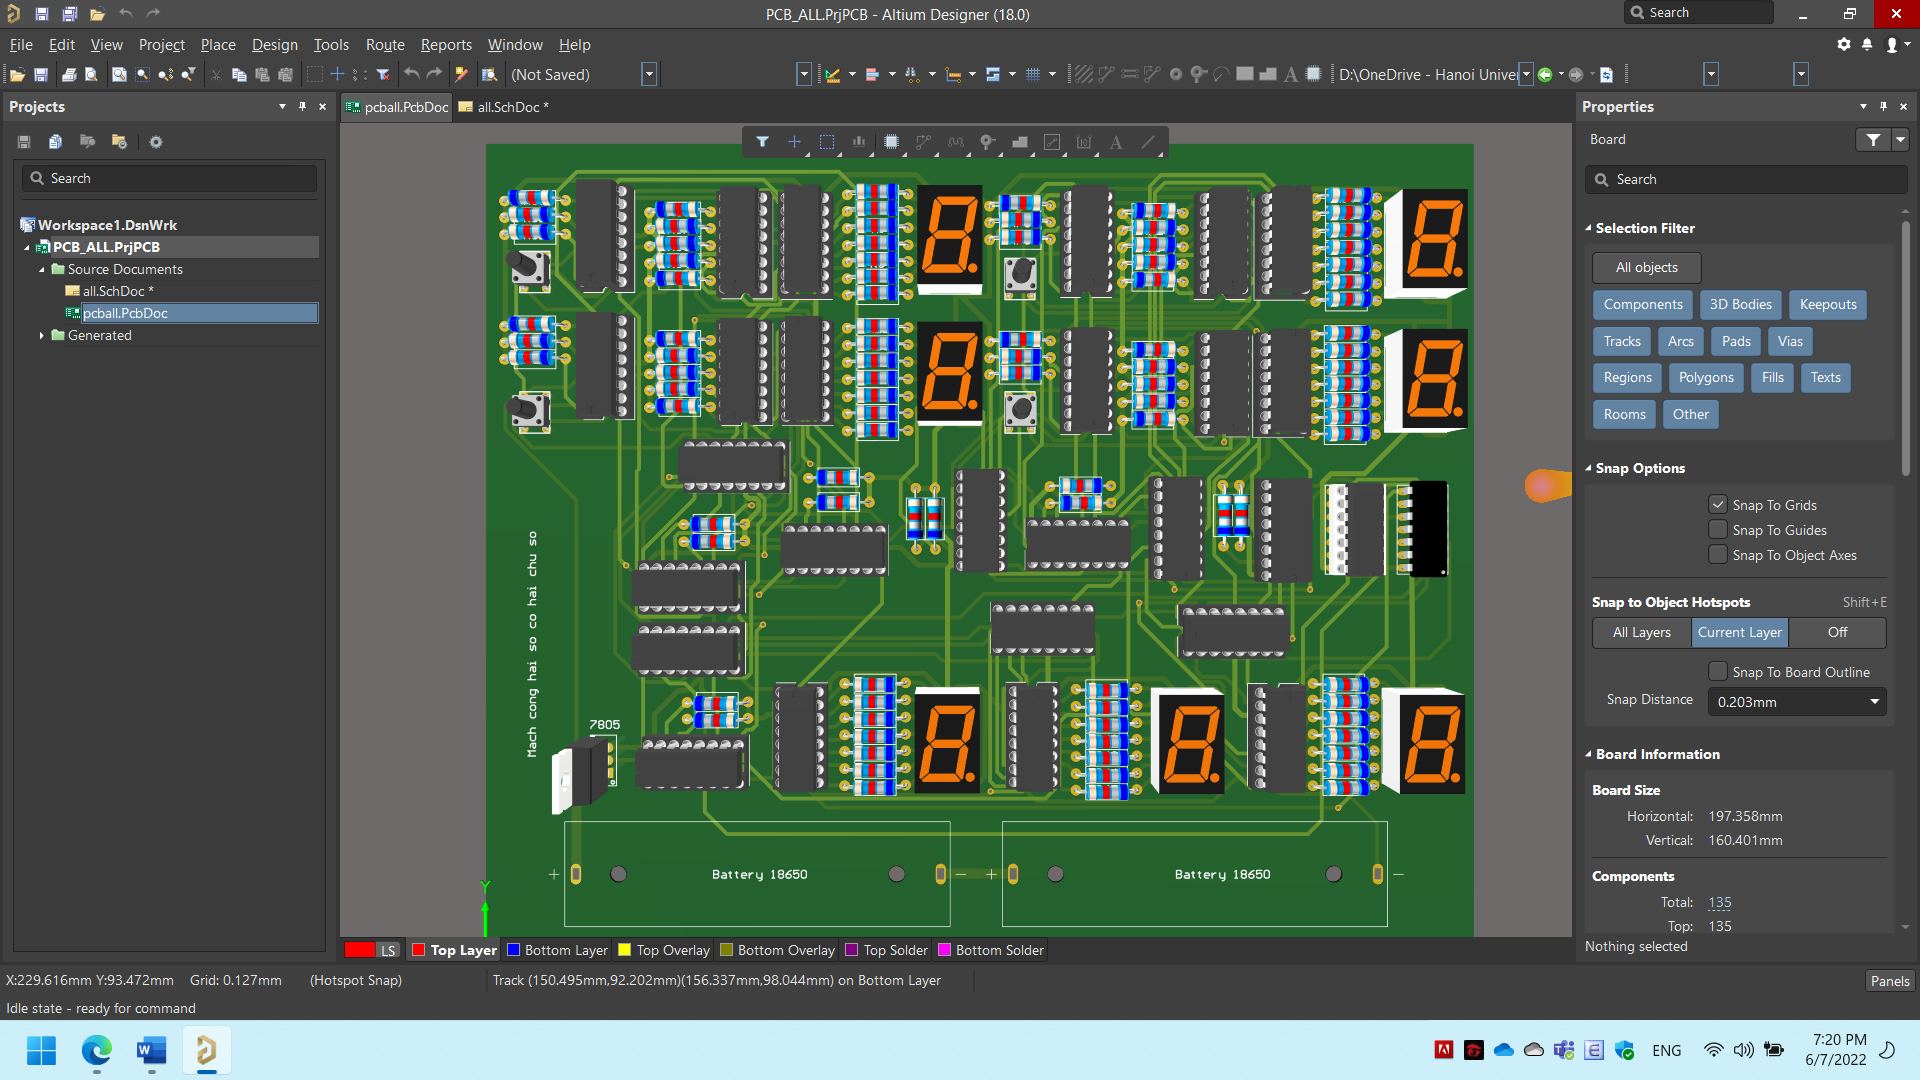
\includegraphics[width=0.8\linewidth]{img_all}\\
		\textit{{Hình ảnh thiết kế mạch trên Altium}}
	\end{center}
\end{frame}

\begin{frame}
	\frametitle{Kết quả}
	\framesubtitle{Gerber mạch gửi đi gia công}
	Do đã sửa lại file mạch mà quên không BackUp lại file cũ nên chỉ còn file Gerber xuất gửi đi gia công.
	\begin{center}
		\includegraphics[width=0.7\linewidth]{image/geber}\\
		\textit{File Gerber}
	\end{center}
\end{frame}

\begin{frame}
	\frametitle{Kết quả}
	\framesubtitle{Mạch thật}
	Do chính sách Zero-Covid của Trung nên không đặt mạch Trung được, đặt mạch Việt Nam nên chất lượng hơi xấu
	\begin{center}
		\includegraphics[width=0.5\linewidth]{image/machin}\\
		\textit{Kết quả mạch in}
	\end{center}
\end{frame}

\subsection{Kết quả thực hiện trên Proteus}
\begin{frame}
	\frametitle{Kết quả}
	\framesubtitle{Kết quả thực hiện trên Protues}
	
	\begin{center}
		\includegraphics[width=1\linewidth]{image/prtfull4}\\
		\textit{Thực hiện phép tính trên Proteus}
	\end{center}
\end{frame}
\subsection{Kết quả thực hiện trên mạch thật}
\begin{frame}
	\frametitle{Kết quả}
	\framesubtitle{Kết quả thực hiện trên mạch thật}
	
	\begin{center}
		\includegraphics[width=0.65\linewidth]{image/real}\\
		\textit{Thực hiện phép tính trên mạch thật}
	\end{center}
	
\end{frame}

\section{Gỡ lỗi, hiệu chỉnh và cải tiến}\subsection{Lỗi về nguồn}
\begin{frame}
	\frametitle{Gỡ lỗi, hiệu chỉnh và cải tiến}
	\framesubtitle{Lỗi về nguồn}
	
	\begin{itemize}
		\item Sử dụng 2 pin 18650 $\to U \approx 8V$, qua ổn áp bằng IC7805, tuy nhiên IC không chịu được dòng lớn, và quá tải.
		\item  Sử dụng 2 pin 18650 $\to U \approx 8V$, không qua ổn áp, gây ra dòng lớn ~1.2A, các đường dây bị nóng, IC, trở bị nóng. Điều này giảm tuổi thọ cho IC.
		\item  Sử dụng 1 pin 18650, $\to U \approx 4.2V$, mạch hoạt động bình thường ở điện áp thấp hơn điện áp định mức. Tuy nhiêm, sụt áp không đáng kể và các điện áp mức cao khi đến chân IC vẫn lớn hơn 3.3V
	\end{itemize}
	Tại sao không tăng áp lên 5V hay sử dụng Adapter? \\$\to$ Tại vì hết kinh phí thực hiện 
\end{frame}
	\subsection{Lỗi đi dây trong mạch}
\begin{frame}
	\frametitle{Gỡ lỗi, hiệu chỉnh và cải tiến}
	\framesubtitle{Lỗi đi dây trong mạch}

	\begin{multicols}{2}
		\begin{center}
			\includegraphics[width=0.7\linewidth]{image/bug1}
		\end{center}
		\begin{center}
			\includegraphics[width=0.7\linewidth]{image/bug2}
		\end{center}
		\begin{center}
			\includegraphics[width=0.7\linewidth]{image/bug5}
		\end{center}
		\begin{center}
			\includegraphics[width=0.7\linewidth]{image/bug4}
		\end{center}
	\end{multicols}
\end{frame}
	\subsection{Sai Schematic}
\begin{frame}
	\frametitle{Gỡ lỗi, hiệu chỉnh và cải tiến}
	\framesubtitle{Lỗi sai Schematic trong quá trình mô phỏng không phát hiện ra}

	Trong quá trình mô phỏng, tại xử lý bit bị tràn đã quên đi mất phải OR bit bị tràn và bit lớn hơn bằng 10 với nhau để tạo ra bit số hàng trăm. Đây là một lỗi dễ sửa, chỉ cần sử dụng con OR còn lại trong IC 74HC32 để làm phép tính là có thể ra được bit đưa vào hàng trăm
	\begin{multicols}{2}
		\begin{center}
			\includegraphics[width=0.7\linewidth]{image/bug3}\\
			\textit{Đi dây lại cho 74HC32}
		\end{center}
	\hfill\null\columnbreak
	\begin{center}
		\includegraphics[width=0.7\linewidth]{image/bug6}\\
		\textit{Sử dụng thêm partD của IC để thực hiện phép OR còn lại}
	\end{center}
	
	\end{multicols}
\end{frame}
	\subsection{Mạch Flip Flop hoạt động không ổn định}
\begin{frame}
	\frametitle{Gỡ lỗi, hiệu chỉnh và cải tiến}
	\framesubtitle{Mạch Flip Flop hoạt động không ổn định}

	Mạch Flip Flop hoạt động không ổn định có các nguyên nhân sau:
	\begin{itemize}
		\item Chân IC bị lỏng, IC kém chất lượng, gây ra nhiễu trong quá trình sử dụng. Trong quá trình kiểm tra, có những lúc Q và $\overline{Q}$ có cùng mức logic nhưng 2 chân này không thông mạch.
		\item Do nhấn nút không dứt khoát, gây ra việc tạo nhiều xung trong một lần nhấn
	\end{itemize}
\begin{multicols}{2}
	\begin{center}
		\includegraphics[width=0.65\linewidth]{image/bug7}
	\end{center}
	\newpage
	$\to$ Các xung xuất hiện trong thời gian rất ngắn, trong khi thiết bị không đủ nhạy, mắt người không đủ khả năng để quan sát nên rất khó phát hiện.\\
	Hình ảnh bên là một lần may mắn thu lại được tín hiệu
\end{multicols}
\end{frame}


\section{Thống kê chi phí}
\begin{frame}
	\frametitle{Thống kê chi phí}
	\begin{center}
		\begin{tabular}{|c|c|c|c|}
			\hline
			\textbf{Linh kiện} & \textbf{Số lượng} & \textbf{Đơn giá} & \textbf{Thành tiền} \\
			\hline
			Bo mạch in & 1 & 510.000 & 510.000 \\
			\hline
			74LS247 & 7 & 25.000 & 175.000 \\
			\hline
			74LS76 & 8 & 7.000 & 56.000 \\
			\hline
			74LS83 & 5 & 10.000 & 50.000 \\
			\hline
			74LS85 & 6 & 10.000 & 60.000 \\
			\hline
			74HC32 & 1 & 4.000 & 4.000 \\
			\hline
			74HC04 & 1 & 5.000 & 5.000 \\
			\hline
			LED 7 SEG & 7 & 4500 & 31.500 \\
			\hline
			Đế IC & 28 & 500 & 14\\
			\hline
			Đế pin, button, ... & --- & 10.000 & 10.000 \\
			\hline
			Tổng cộng & 36 & --- & \color{red}\textbf{915.500}\color{black}\\
			\hline
		\end{tabular}
	\end{center}
$\to$ Đây mới chỉ là chi phí tính trên bo mạch khi thành công, chi phí thất bại chưa tính
\end{frame}




\begin{frame}{}
	\centering \LARGE
	\emph{Thank you!!}
\end{frame}



\end{document}